\documentclass{article}  % Define la clase del documento.

% Paquetes de idioma y codificación
\usepackage[utf8]{inputenc}
\usepackage[T1]{fontenc}
\usepackage[spanish]{babel}  % Ajusta el idioma del documento a español.

% Paquete de geometría para configurar márgenes y tamaño de papel
\usepackage[letterpaper, margin=3cm]{geometry}

% Paquetes de tipografía
\usepackage{mathptmx}    % Usa Times New Roman como fuente.
\usepackage{microtype}   % Mejora la justificación del texto.

% Paquetes para manejo de colores y gráficos
\usepackage{xcolor}      % Define y utiliza colores.
\usepackage{graphicx}    % Permite la inserción de imágenes.
\usepackage{tikz}        % Creación de gráficos vectoriales.

% Configuración de enlaces y referencias cruzadas
\usepackage{hyperref}
\hypersetup{
    colorlinks   = true,
    linkcolor    = darkblue,
    citecolor    = black,
    filecolor    = blue,
    urlcolor     = blue
}

% Paquetes para la mejora visual de tablas y figuras
\usepackage{booktabs}    % Para tablas de alta calidad.
\usepackage{float}       % Controla la posición de figuras y tablas.

% Paquete para la personalización de códigos fuente
\usepackage{listings}
\lstset{
    literate=
    {á}{{\'a}}1 {é}{{\'e}}1 {í}{{\'i}}1 {ó}{{\'o}}1 {ú}{{\'u}}1
    {Á}{{\'A}}1 {É}{{\'E}}1 {Í}{{\'I}}1 {Ó}{{\'O}}1 {Ú}{{\'U}}1
    {ñ}{{\~n}}1 {Ñ}{{\~N}}1 {ü}{{\"u}}1 {Ü}{{\"U}}1,
    backgroundcolor=\color{backcolour},
    commentstyle=\color{codegreen},
    keywordstyle=\color{codepurple},
    numberstyle=\tiny\color{codegray},
    stringstyle=\color{red},
    basicstyle=\ttfamily\small,
    breakatwhitespace=false,
    breaklines=true,
    captionpos=b,
    keepspaces=true,
    numbers=left,
    numbersep=5pt,
    showspaces=false,
    showstringspaces=false,
    showtabs=false,
    tabsize=2,
    language=TeX,
    morecomment=[l]\#,
    frame=single,
    rulecolor=\color{black}
}

% Definición de colores al estilo Visual Studio Code
\definecolor{darkblue}{rgb}{0.0, 0.0, 0.55}  % Enlaces
\definecolor{codegreen}{rgb}{0.25, 0.49, 0.48}  % Comentarios
\definecolor{codegray}{rgb}{0.5, 0.5, 0.5}  % Números y anotaciones
\definecolor{codepurple}{rgb}{0.58, 0, 0.82}  % Palabras clave
\definecolor{backcolour}{rgb}{0.95, 0.95, 0.92}  % Fondo de código

% Configuraciones de párrafo y matemáticas
\usepackage{amsmath}
\usepackage{parskip}    % Espaciado entre párrafos.
\usepackage{ragged2e}   % Justificación mejorada.

% Configuración de secciones y encabezados
\usepackage{titlesec}
\titleclass{\part}{top} % Make part like a class
\titleformat{\part}[display]
  {\normalfont\huge\bfseries\centering}{\thepart}{20pt}{\Huge}
\titlespacing*{\part}{0pt}{-60pt}{10pt}
\titleformat{\part}
  {\normalfont\huge\bfseries}{}{0pt}{}

% Asegúrate de usar esto para mantener el estilo en las páginas de las partes
\titleformat{\part}[display]
  {\normalfont\huge\bfseries}{}{0pt}{}
  [\thispagestyle{fancy}] % Aplica el estilo fancy a las páginas de las partes

% Configuración de encabezados y pies de página personalizados
\usepackage{fancyhdr}
\pagestyle{fancy}
\fancyhf{}
\fancyhead[L]{\raisebox{0.20cm}{\textbf{Apuntes Prueba 1 Hidrologia}}}
\fancyhead[R]{\raisebox{0.1cm}{
\includegraphics[width=0.25\linewidth]{LOGO_UNIVERSIDAD.jpg}}}
\fancyhead[C]{\rule{\textwidth}{0.6pt}}
\fancyfoot[C]{\rule{\textwidth}{0.6pt}}
\fancyfoot[R]{\raisebox{-1.5\baselineskip}{\thepage}}
\renewcommand{\headrulewidth}{0pt}
\renewcommand{\footrulewidth}{0pt}

% Configuración avanzada de geometría
\geometry{
  top=3.5cm, % Aumenta el espacio en la parte superior para subir el encabezado
  bottom=2.5cm,
  headheight=2.5cm % Aumenta la altura del encabezado si es necesario
}

% Configuracion de bibliografia
\usepackage{natbib}
\bibliographystyle{unsrtnat}  % Puedes cambiarlo por `unsrtnat`, `abbrvnat`, etc.

\begin{document}
%----------------------------------------------------------------------------------------
% PORTADA
%----------------------------------------------------------------------------------------
\begin{titlepage}%Inicio de la carátula, solo modificar los datos necesarios
\newcommand{\HRule}{\rule{\linewidth}{0.5mm}} 
\center 
%----------------------------------------------------------------------------------------
%	ENCABEZADO
%----------------------------------------------------------------------------------------

\includegraphics[width=10cm]{LOGO_UNIVERSIDAD.jpg}\\ % Si esta plantilla se copio correctamente, va a llevar la imagen del logo de la facultad.OBS: Es necesario incluir el paquete: graphicx
\vspace{3cm}
%----------------------------------------------------------------------------------------
%	SECCION DEL TITULO
%----------------------------------------------------------------------------------------
\HRule \\[0.4cm]
{ \huge \bfseries Apuntes Prueba 1}\\[0.4cm] % Titulo del documento
{ \huge \bfseries Hidrologia}\\[0.4cm] % Titulo del documento
\HRule \\[1.5cm]
 \vspace{5cm}
%----------------------------------------------------------------------------------------
%	SECCION DEL AUTOR
%----------------------------------------------------------------------------------------
\begin{flushright}
    { 
    \textbf{Autores:} \\
    Lukas Wolff Casanova\\
}
\end{flushright}
\vspace{1cm}
%----------------------------------------------------------------------------------------
%	SECCION DE LA FECHA
%----------------------------------------------------------------------------------------
{\large \textbf{\today}}\\[2cm] % El comando \today coloca la fecha del dia, y esto se actualiza con cada compilacion, en caso de querer tener una fecha estatica, reemplazar el \today por la fecha deseada
\end{titlepage}
%----------------------------------------------------------------------------------------
%  INDICE
%----------------------------------------------------------------------------------------
\newpage
\thispagestyle{empty} % Deshabilita el número de página en la página del índice
\tableofcontents
\thispagestyle{plain} % Deshabilita el encabezado en la página del índice
\thispagestyle{empty} % Deshabilita el número de página en la página del índice
\newpage

%\newpage
%\thispagestyle{empty}
%\listoffigures 
%\thispagestyle{plain} % Deshabilita el encabezado en la página del índice %
%\thispagestyle{empty}
%\newpage
%----------------------------------------------------------------------------------------
%ACÁ EMPIEZA EL INFORME
\setcounter{page}{1}
%----------------------------------------------------------------------------------------
\part{Capitulo 7}

\section{Tipos de Equipos}

\begin{itemize}
    \item Movimiento de Tierras
    \begin{itemize}
        \item Excavadoras (orugas con pala frontal)
        \item Buldozer
        \item Camion Tolva
        \item Retro Excavadora (Pala delantera y brazo atras)
        \item Mononiveladora (Niveladora de caminos)
        \item Motoniveladora (Igual pero con motor)
        \item Cargador Frontal (Pala frontal grande con articulacion en vehiculo y no en las ruedas)
        \item Mototrailla o Trailla (Permite ditribuir tierra)
    \end{itemize}
    \item Compactacion o Nivelacion
    \begin{itemize}
        \item Placa Compactadora (Se usa manualmente)
        \item Rodillo compactador liso (Hay de distintos tamaños)
        \item Rodillo compactador pata de cabra (Se usa para compactar mas profundamente)
        \item Rodillo compactador neumatico (Se usa para compactar asfalto, el que tiene muchas ruedas)
    \end{itemize}
    \item Produccion de Hormigon, existen distintos tipos de maquinas o instalaciones
\end{itemize}

\textbf{Criterios de Seleccion:} Se debe considerar el costo total, lo que comprende la inversion original mas el costo de operacion, costo de reparacion y mantencion del equipo. La suma de todo esto se define como \textbf{INVERSION TOTAL DE UN EQUIPO}

\section{Productividad de Equipos}

De este modo, se busca la productividad optima \textbf{Qp} la cual se basa en la operacion continua de la maquinaria por hora. Se define la productividad normal \textbf{Qv} como Qv incorporando el factor humano (0.85). Ademas si se agrega el factor de direccion del trabajo (fp), se optiene la productividad real \textbf{Qr}

\begin{equation}
    Qr = fp \cdot Qn = fp \cdot fw \cdot Qp = fa \cdot Qp
\end{equation}

\newpage
\section{Costos de Equipos}

Hay que tomar en consideracion costos como depreciacion e inversion inicial:

\begin{figure}[H]
    \centering
    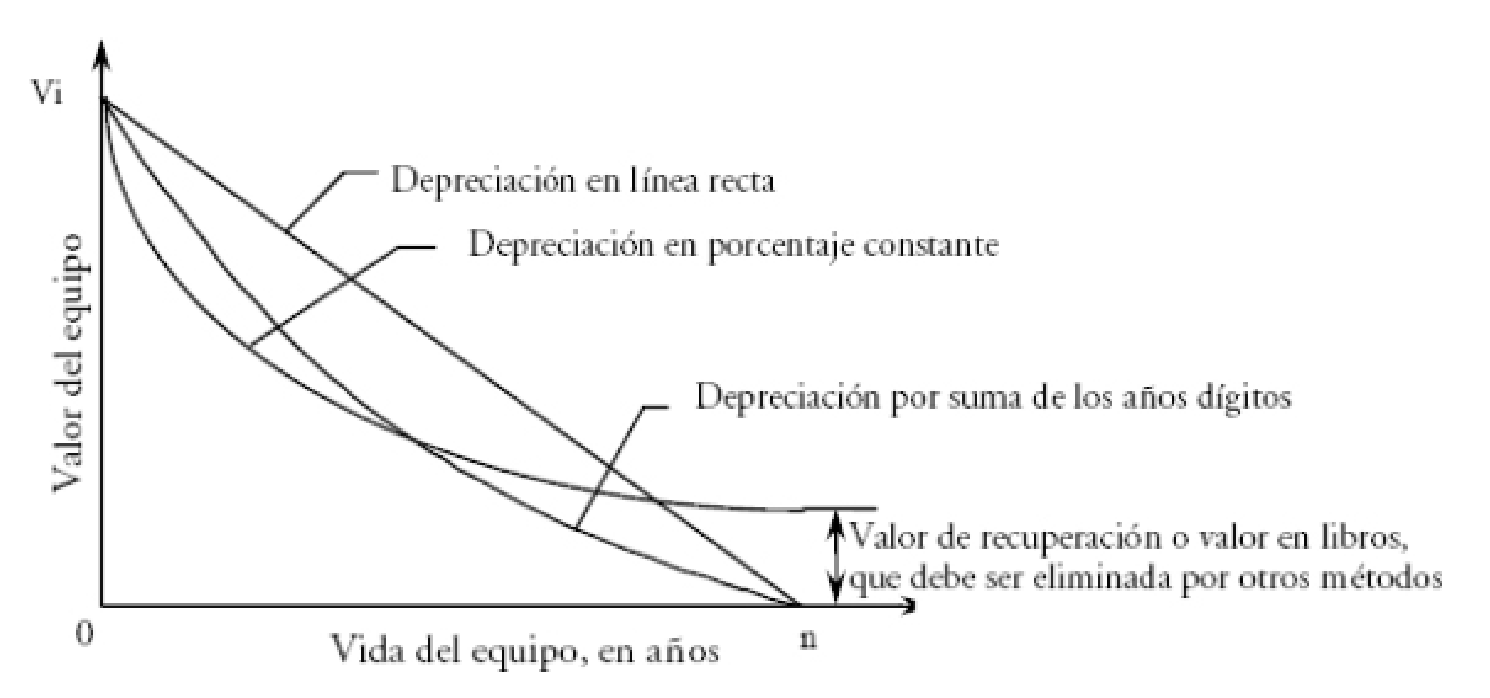
\includegraphics[width=0.8\linewidth]{FOTOS/costo_equipo.png}
    \caption{Costos de Equipos}
    \label{fig:costos}
\end{figure}

\begin{itemize}
    \item Costos de inversion
    \begin{itemize}
        \item Compra 
        \item Internacion
        \item Flete
        \item Seguro de traslado
        \item Intereses
        \item Impuestos
        \item Seguro
        \item Almacenaiento
    \end{itemize}
    \item Costos de operacion
    \begin{itemize}
        \item Operador
        \item Combustible
        \item Lubricacion
        \item mantencion
        \item Reparaciones menores
        \item Neumaticos y Filtros
    \end{itemize}
\end{itemize}

\newpage
\section{Vida Equipo}

De esta forma, la vida de un equipo se define como:

\begin{figure}[H]
    \centering
    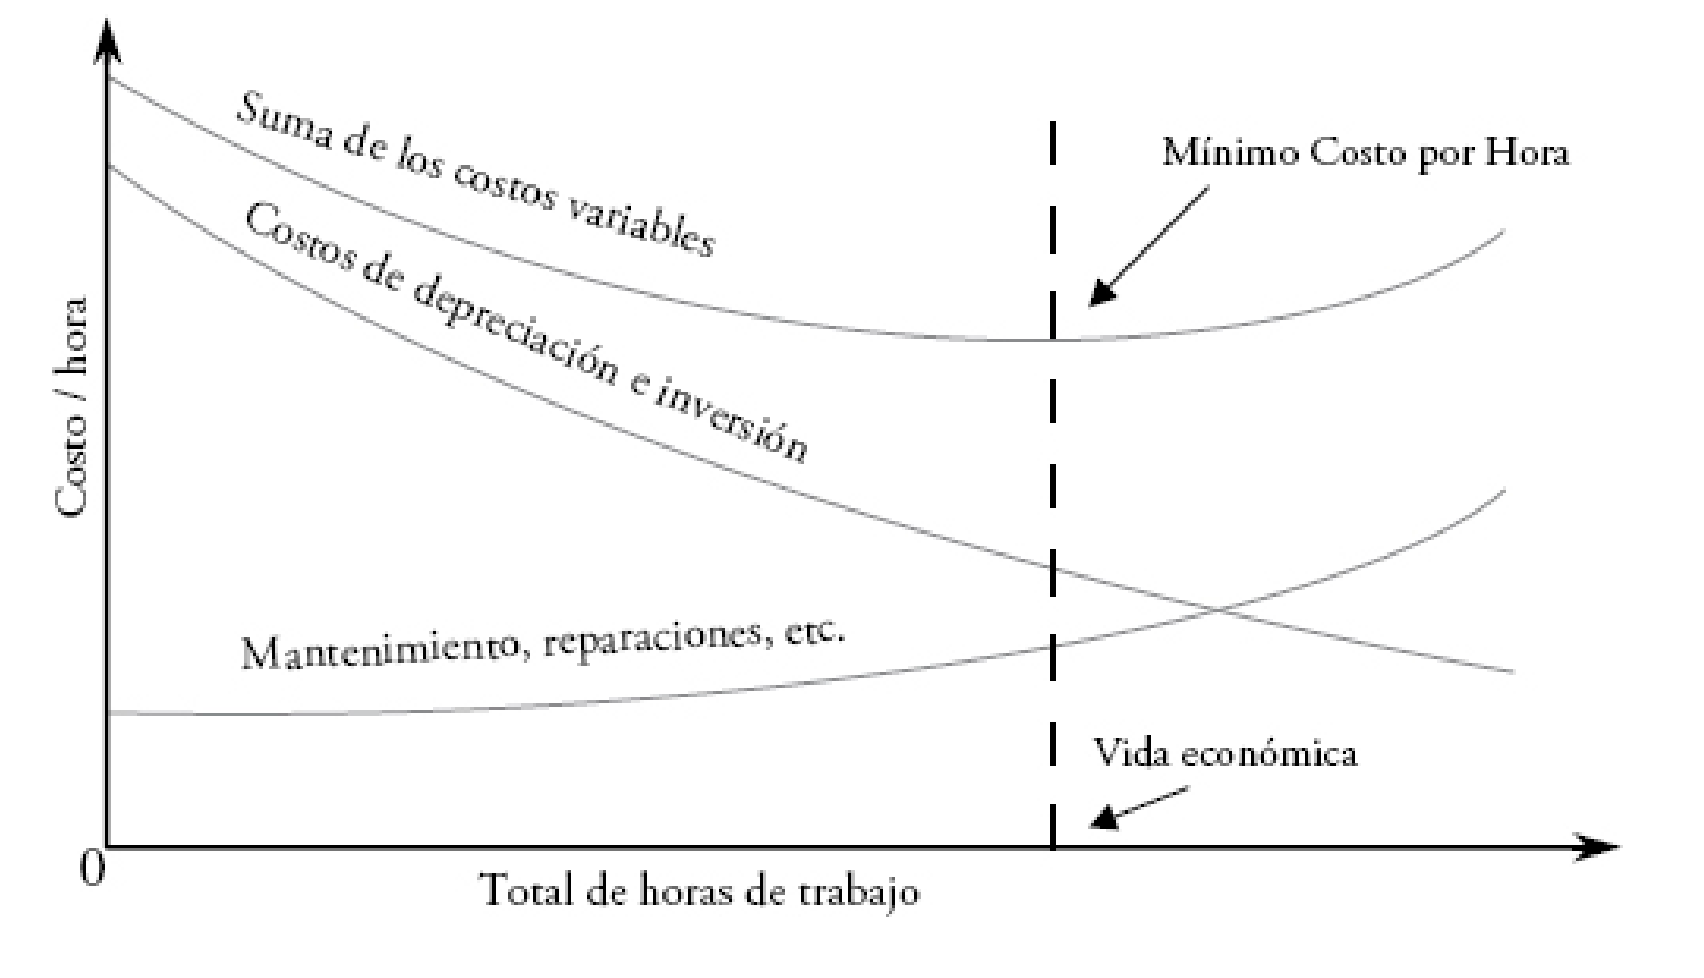
\includegraphics[width=0.8\linewidth]{FOTOS/vida_equipo.png}
    \caption{Vida de un Equipo}
    \label{fig:vida}
\end{figure}

\part*{Capítulo 8}

\section{Movimiento de tierra}
\begin{itemize}
    \item Desmalezar el terreno
    \item Remover estructuras y árboles existentes
    \item Nivelar el terreno
    \item Señalizar las obras y colocar protecciones
    \item Planificar la circulación de vehículos, maquinarias y personas
    \item Planificar el retiro de escombros
    \item Proteger estructuras y árboles existentes
    \item Determinar las técnicas a emplear para la evacuación de agua subterránea o de superficie
    \item Precauciones especiales con el medio ambiente
\end{itemize}

Antes de iniciar cualquier obra, es necesario replantear los planos en el terreno, marcando referencias que permitan verificar distancias, cotas y ángulos durante la excavación y construcción. Tras las excavaciones, se debe verificar nuevamente el replanteo. En grandes movimientos de tierra, se recomienda escarificar la capa superficial (10 a 20 cm) y almacenarla para reutilizarla. Esto evita la importación de material y ayuda a recuperar semillas y microorganismos locales, favoreciendo un equilibrio ambiental más rápido.

Una excavación puede hacerse empleando variadas técnicas, según las condiciones del proyecto y las restricciones específicas. Algunas son:
\begin{itemize}
    \item Tipo de proyecto de ingeniería.
    \item Tamaño y profundidad de la excavación.
    \item Tipo de terreno (roca o suelo, tipo de estratificación, etc.).
    \item Calidad del suelo (inclinación de taludes o protecciones).
    \item Estructuras contiguas.
    \item Restricciones de espacio.
    \item Equipo y maquinaria disponible.
    \item Presencia de agua subterránea o superficial.
    \item Condiciones ambientales.
\end{itemize}

En trabajos pequeños y en suelo blando, la tierra se puede excavar con palas y picota si se requiere. En excavaciones abiertas con volúmenes mayores de movimiento de tierra se debe considerar el empleo de equipos especializados, como:
\begin{itemize}
    \item Palas Mecánicas: cargadores frontales, retroexcavadoras, palas frontales.
    \item Dragas.
    \item Grúas con cucharón de almeja.
    \item Zanjadoras y otros.
\end{itemize}

\begin{itemize}
    \item \textbf{Excavación de zapata}: Excavación de dimensiones similares (largo, ancho y profundidad).
    \item \textbf{Excavación en zanja}: Excavación larga y angosta (ancho entre 0.5 m y 3.2 m) para fundaciones corridas o canalizaciones.
    \item \textbf{Excavaciones amplias}: Excavaciones de más de 3.2 m de ancho, usadas para subterráneos y grandes fundaciones.
    \item \textbf{Pozos}: Excavaciones profundas y de forma rectangular o circular, para captación de agua o prospección de suelos.
\end{itemize}

Una excavación abierta se puede diseñar de las siguientes formas:
\begin{itemize}
    \item \textbf{Taludes libres}: vertical, inclinado, escalonado.
    \item \textbf{Taludes protegidos}: apuntalados, entibados.
\end{itemize}

Los factores y condiciones especiales de la obra que lo condicionan son:
\begin{itemize}
    \item Tipo de terreno.
    \item Costo relativo entre ambas soluciones.
\end{itemize}

Los factores que condicionan la excavación son:
\begin{itemize}
    \item \textbf{Tiempo de apertura}: Si es prolongado, es recomendable proteger los taludes, especialmente en zonas sísmicas o con vibraciones.
    \item \textbf{Asentamientos permisibles} alrededor de la excavación.
    \item \textbf{Presencia de agua}.
\end{itemize}

\textbf{Excavaciones con talud libre}: Para excavaciones mayores a 1.2 m de profundidad, si el terreno es cohesivo y permite un talud vertical, se puede realizar sin entibación si se ha calculado la altura crítica de excavación (Hc). La ecuación para Hc es:

\[
Hc = 1.3 \frac{q_u}{\gamma}
\]

donde:
\begin{itemize}
    \item $qu$: resistencia al corte de una muestra de suelo, en kg/m².
    \item $\gamma$: densidad natural del terreno, en kg/m³.
\end{itemize}

Esta fórmula es válida si cualquier sobrecarga en el borde de la excavación está a una distancia mayor que la profundidad de la excavación (Hs).


\begin{figure}[h]
    \centering
    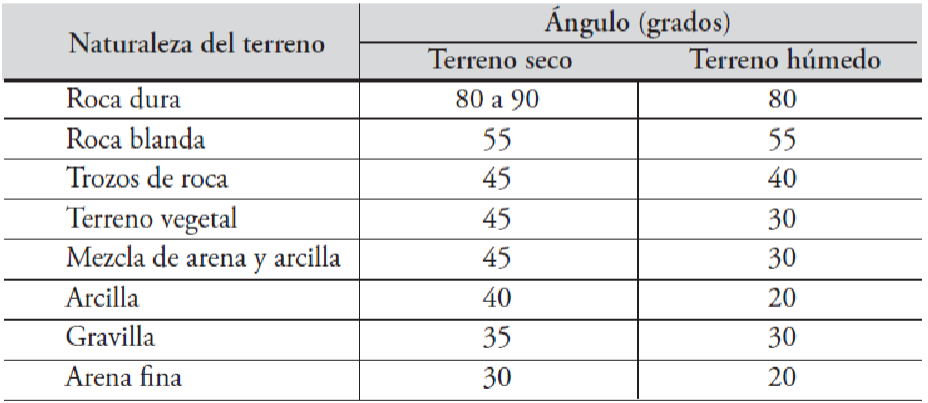
\includegraphics[width=0.8\textwidth]{aaa.png}
    \caption{Recomendaciones de talud libre.}
    \label{fig:8_1}
\end{figure} 


La altura máxima de excavación, denominada altura de seguridad ($H_s$), se calcula dividiendo la altura crítica $H_c$ por un factor de seguridad (F.S.) entre 1.1 y 2.0:

\[
H_s = \frac{H_c}{F.S.}
\]

Si hay sobrecargas en el borde de la excavación (maquinaria, materiales, etc.), se usará esta fórmula para calcular $H_s$.

\[
Hc = 1.3 \frac{q_u - \sigma}{\gamma}
\]

Se recomienda usar taludes verticales solo en terrenos cohesivos o medianamente cohesivos y en excavaciones de corta duración, ya que el suelo puede perder humedad rápidamente. Una solución intermedia es el uso de taludes escalonados para reducir el volumen de tierra removido.

Los tipos más comunes de protección en excavaciones provisionales son:
\begin{itemize}
    \item Hormigón proyectado o Shotcrete.
    \item Mallas metálicas.
    \item Puntales.
    \item Entibaciones.
\end{itemize}

La presencia de agua en una excavación puede desestabilizar el suelo, causando desprendimientos y socavaciones, además de complicar el trabajo. Las técnicas más utilizadas para manejar el agua son:
\begin{itemize}
    \item Sistemas sin depresión previa de la napa.
    \item Sistemas con depresión previa de la napa.
    \item Sistemas de ataguías.
    \item Sistemas especiales.
\end{itemize}

Si hay estructuras con fundaciones superficiales cercanas a la excavación, cualquier asentamiento puede causar daños. Con una buena entibación, el asentamiento máximo no suele exceder el 0.5\% de la profundidad de la excavación. La magnitud de los movimientos y asentamientos depende de:
\begin{itemize}
    \item Relación ancho-profundidad de la excavación.
    \item Procedimiento constructivo, número y tipo de codales, velocidad de construcción.
    \item Espesor de arcilla blanda bajo el fondo de la excavación.
\end{itemize}

\textbf{Asentamientos y recalzos}: Si junto a la excavación hay fundaciones de estructuras grandes y la profundidad de la excavación supera la cota de fundación de la obra contigua, el cimiento existente debe protegerse o recalzarse. La prolongación de la fundación debe hacerse siguiendo una metodología precisa.


\end{document}
